Wenn Licht auf eine Grenzfläche wie zum Beispiel Glas oder Wasser trifft, ändert die Lichtwelle auf beiden Seiten der Grenzfläche sowohl die Richtung als auch die Ausbreitungsgeschwindigkeit. Dieses Phänomen wird als \textbf{Brechung} bezeichnet und quantitativ über den Brechungsindex $n$ beschrieben 
\begin{align}\label{eq:snellius}
	n = \frac{v_1}{v_2} = \frac{\sin{\alpha_1}}{\sin{\alpha_2}} \quad .
\end{align}
Dieser Zusammenhang wird auch Snelliussches Gesetz genannt. Die Ausbreitungsgeschwindigkeit im jeweiligen Medium ist $v$ und der Eintrittswinkel $\alpha$. \\
Die Brechung ist im Allgemeinen abhängig von der Wellenlänge $\lambda$ des einfallenden Lichtes. Man spricht von \textbf{Dispersion}. \\
Eine, für viele Phänomene hinreichend genaue, Dispersionsrelation wird aus der Maxwellschen Theorie der elektromagnetischen Wellen hergeleitet. Sie gilt für Wellenlängen, bei denen kaum Absorption auftritt. Überlegungen zur Kraft eines Elektrischen Feldes liefern eine inhomogene Differentialgleichung (DGL) zweiter Ordnung, die der einer erzwungenen und gedämpften Schwingung entspricht. Die Anregung erfolgt durch eine ebene elektromagnetische Welle der Form
\begin{align}
	\va{E}_0 e^{i\omega t} \quad.
\end{align}
	Die Reibungskraft dämpft proportional zur Geschwindigkeit und die rücktreibende Kraft hängt von der Auslenkung des Ladungsträgers aus seiner Ruhelage ab
\begin{align}
	m_i \dv[2]{\va{x}_i}{t} + f_i \dv{\va{x}_i}{t} + a_i \va{x}_i = q_i \va{E}_0 e^{i\omega t} \quad .
\end{align}
Diese DGL kann auch über die Polarisation und das damit verbundene Dipolmoment $\va{p_i} = q_i \va{x}_i$ ausgedrückt werden:
\begin{align}
\va{P} = \sum_{i} \va{P}_i = \sum_{i} N_i q_i \va{x}_i \quad.
\end{align}
Die Lösung lautet dann:
\begin{align}
\va{P} = \sum_{i} \frac{1}{\omega_i^2 - \omega^2 + \frac{i f_i \omega}{m_i}} \frac{N_i q_i^2}{m_i} \va{E}_0 e^{i \omega t} \quad .
\end{align}
Der Bezug zum Brechungsindex wird über die dielektische Verschiebung $\epsilon$, eine Material\-eigenschaft, hergestellt
\begin{align}
\va{P} = (\tilde{\epsilon} -1) \epsilon_o \va{E} = (\tilde{n}^2 - 1) \epsilon_0 \va{E}_0 e^{i \omega t} \ , \quad \tilde{\epsilon}, \tilde{n} = n(1-i k) \in \mathbb{C} \quad .
\end{align}
Es folgt
\begin{align}\label{Absorptionsstelle}
\text{Re}\left( \tilde{n}^2 \right) = n^2(1-k^2) = 1 + \sum_{i} \frac{N_i q_i ^2 (\omega_i^2 - \omega^2)}{\epsilon_0 m_i \left((\omega_i^2 - \omega^2)^2 + \frac{f_i^2}{m_i^2} \omega^2 \right)}  \quad.
\end{align}
Aus der Forderung, dass die Gleichung nur gelten soll, wenn der Absorptionskoeffizient $k$ verschwindet folgt wiederum direkt
\begin{align}
\text{Im}\left( \tilde{n}^2 \right) = -2 n^2 k = 0 \rightarrow f_i = 0
\end{align}
und demnach
\begin{align} \label{eq:dispersionsrelation}
n^2(\omega) = 1 + \sum_{i} \frac{N_i q_i^2}{\epsilon_0 m_i} \frac{1}{\omega^2 - \omega_i^2}  \quad.
\end{align}
\clearpage

In Gleichung \eqref{eq:dispersionsrelation} wird noch die Windelgeschwindigkeit $\omega$ durch die Observable, die Wellenlänge $\lambda  = \frac{2 \pi c}{\omega}$ ersetzt, um sie dann in eine Potenzreihe zu entwickeln. \\
Hierbei werden zwei Fälle unterschieden: Ist die Wellenlänge größer oder kleiner als die Absorptionsstelle $\lambda_1$. Es wird davon ausgegangen, dass nur eine solche Absorptionsstelle vorliegt. \\
\underline{Fall 1 $(\lambda \gg \lambda_1)$ :}  \\
\begin{align}\label{Fall1}
n^2(\lambda) = A_0 + \frac{A_2}{\lambda^2} + \frac{A_4}{\lambda^4} + ... \ , \quad A_0, A_2, A_4 > 0
\end{align}
\underline{Fall 1 $(\lambda \ll \lambda_1)$ :}  \\
\begin{align}\label{Fall2}
n^2(\lambda) = 1 + A'_2 \lambda^2 + A'_4 \lambda^4 + ... \ , \quad A'_2, A'_4 > 0
\end{align}
Die beiden Dispersionskurven stellen die normale Dispersion dar. Das bedeutet, dass der Brechungsindex mit zunehmender Wellenlänge abnimmt. Die beiden Fälle unterscheiden sich jedoch in der Krümmung. Abbildung~\ref{fig:dispersionskurven} zeigt Fall 1 in a) und Fall 2 in b).

\begin{figure}[h!]
	\centering
	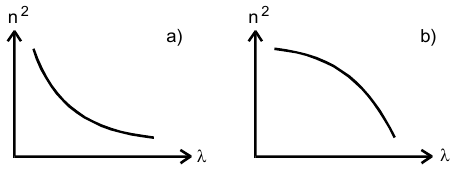
\includegraphics[width=0.7\textwidth]{Theorie.png}
	\caption{Dispersionskurven\footnotemark}
	\label{fig:dispersionskurven}
\end{figure}
\footnotetext{Versuchsanleitung V402: \url{http://129.217.224.2/HOMEPAGE/Anleitung_AP.html}}